\documentclass{book}
\usepackage{mathtools}
\usepackage{tikz}
\usetikzlibrary{positioning}

\usepackage{amsthm}
\usepackage{amsmath}
\usepackage{amssymb}

\newtheorem{defn}[equation]{Definition}
\newtheorem{coro}[equation]{Corollary}
\newtheorem{prop}[equation]{Proposition}
\renewenvironment{proof}{\emph{Proof}}{\qed}


\begin{document}

\tableofcontents


Think about a new outline: 
- Introduce quantities, manifolds, etc. as before. 
- vector as infinitesimal displacement/"line"
- Outer product and K-vectors and infinitesimal K-surfaces
- K-forms as functions of k-vectors
- Integration
- Stokes theorem in diff form
Ch 3
- Symplectic geom (form, ...)
- Riem geom (Inner product, ..)
- ???


\chapter{Mathematical representations of physical objects}


\section{Manifolds and continuous quantities}

\subsection{Summary}

In mathematical science, our goal in general is to be able to assign a numerical value to a physical property of some object. There also ought to be no question of repeatability: two systems prepared identically and measured identically must give the same result (\emph{reference quantum mechanics??}). This directly gives us \textbf{quantities} as functions that assign real values to physical objects. We then group quantities into sets, requiring those sets to be sufficient to distinguish one physical object from another, and calling those sets \textbf{coordinate systems}. Varying a quantity while keeping the others fixed gives us \textbf{coordinate lines}, and because certain physical properties can be equally well described in different coordinate systems, we introduce \textbf{coordinate transformations}. All of these mathematical constructions together, along with the requirement that the set of possible measured values must be completely covered by subsets with defined quantities, gives us \textbf{manifolds}. 

Within manifolds may lie smaller manifolds: \textbf{submanifolds}, or \textbf{k-surfaces}. Having a notion of certain points existing on a submanifold and certain points existing outside of it gives us the notion of the \textbf{interior} of a surface. The \textbf{boundary} of a surface follows naturally as being the set of points on that surface that are not on the interior, and therewith also the \textbf{boundary operator}, which takes us from a k-surface to its boundary. 

We now want to be able to talk about functions along our k-surfaces. We define then \textbf{k-functionals} as linear functions along our k-surfaces. Because of our requirement of linearity, we will be able to start talking about functions over infinitesimals in Chapter 2. Finally, we introduce the \textbf{interior operator}, which applied to a k-functional is equivalent to applying a boundary operator to a (k+1)-surface, and will allow us to talk about Stoke's Theorem in Chapter 2.  


\subsection{Physical objects and quantities}


Our goal in general is to be able to identify and describe physical objects through measurement and experiment. 
Say we're looking at weather. We'll want to know the temperature, wind speed, humidity, whereabouts, etc.

- \emph{We can give real number values describing that object. This gives us quantities}

Fahrenheit, mph, percent humidity, location.
On some set of all possible weather configurations, we look at a specific subset of possibilities described by real numbers. This is our weather report.  

 

\begin{defn}
	A \textbf{quantity} is a function $q : U \to \mathbb{R}$ that assigns a measurable value to a physical object.
\end{defn}


- \emph{Having a set of one-to-one quantities sufficient to distinguish one object from another, but not so many that some end up redundant, gives us a coordinate system}
In identifying them, it is necessary that we are able to distinguish between different objects by those measurable properties. 

\begin{defn}
	A \textbf{coordinate system} $Q$ is a collection of $n$ quantities $q^i : U \to \mathbb{R}^n$ such that there is a one-to-one relationship between the physical objects in $U$ and elements of $\mathbb{R}^n$.
\end{defn}


\begin{defn}
	A \textbf{coordinate line} is the set of points in $\mathbb{R}^n$ obtained by allowing one quantity to vary and holding the others fixed. 
\end{defn}




- \emph{\textbf{Overlapping} coordinate systems can be transformed between}

Moscow may be seen on both a map of Europe and a map of Asia, so its coordinate system can be swapped. Lisbon, however, will not show up on a map of Asia, so its coordinate system cannot be swapped. 

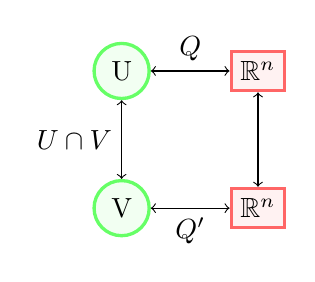
\begin{tikzpicture}
[roundnode/.style={circle, draw=green!60, fill=green!5, very thick, minimum size=7mm},
squarednode/.style={rectangle, draw=red!60, fill=red!5, very thick, minimum size=5mm},
]
\node[roundnode]	(U) {U};
\node[roundnode]	(V) [below=of U]{V};
\node[squarednode]	(realU) [right=of U] {$\mathbb{R}^n$};
\node[squarednode]	(realV) [right=of V] {$\mathbb{R}^n$};

\draw[<->] (U) -- (realU) node[midway, above] {$Q$};
\draw[<->] (U) -- (V) node[midway, left] {$U\cap V$};
\draw[<->] (V) -- (realV) node[midway, below] {$Q'$};
\draw[<->] (realU) -- (realV);
\end{tikzpicture}

\begin{defn}
	Given two coordinate systems  $Q : U \to \mathbb{R}^n$ and $Q' : V \to \mathbb{R}^n$ such that $U \cap V \neq \emptyset$, we call a \textbf{coordinate transformation} the function $f = Q' \circ (Q)^{-1} : \mathbb{R}^n \to \mathbb{R}^n$.
\end{defn}




- \emph{Now that we have sets that can be mapped to the real numbers, we can define manifolds}

For the weather example, a manifold would be all possible weather conditions with a subsection whereon is defined a weather report, measuring temperature, wind speed, etc. in different places. If we're looking to parametrize the entire earth, then our manifold cannot be covered with a single subset, because the earth has poles. We will need multiple subsets to cover all of the earth, and all possible weather conditions. 

Talking about location on the earth, a \textbf{single space cannot cover the entire earth such that a consistent set of quantities will be defined}. The poles must be in two separate subsets, with separate quantities.
 
\begin{defn}
	A \textbf{manifold} is a set of physical objects $X$ such that for any $x \in X$ there exists a $U \subset X$ that contains $x$ and upon which a coordinate system $Q$ is defined.
\end{defn}



\subsection{Sub-manifolds and k-surfaces}

- \emph{Within a manifold can lie a manifold of equal or smaller dimension, with a mapping between them}

If in the original weather report we were worrying about temperature, humidity, and wind speed, we could instead hold one of the three values fixed (say, humidity), and vary the other two. The latter manifold, with humidity held constant, would be a sub-manifold of the former, where all three variables are allowed to change.  



\begin{defn}
	Consider a manifold X of dimension n, and a manifold Y of dimension k, such that $k \leq n$. Y is a \textbf{submanifold} or a k-surface of X if any point on Y is also a point on X. 
\end{defn}

- parameterization of Y can be done in terms of the coordinates of X; $q^i(q'^j)$



\begin{tikzpicture}
[roundnode/.style={circle, draw=green!60, fill=green!5, very thick, minimum size=7mm},
squarednode/.style={rectangle, draw=red!60, fill=red!5, very thick, minimum size=5mm},
]
\node[roundnode]	(X) {X};
\node[roundnode]	(Y) [below=of X]{Y};
\node[squarednode]	(realX) [right=of X] {$\mathbb{R}^n$};
\node[squarednode]	(realY) [right=of Y] {$\mathbb{R}^n$};

\draw[<->] (X) -- (realX) node[midway, above] {$Q$};
\draw[->] (X) -- (Y) node[midway, left] {$U\cap V$};
\draw[<->] (Y) -- (realY) node[midway, below] {$P$};
\draw[->] (realU) -- (realV);
\end{tikzpicture}

What are the possible submanifolds of a given manifold?


\begin{defn}
	For some manifold X of dimension n, $S^k$ is the set of all possible \textbf{k-surfaces}, or sub-manifolds of dimension $k \leq n$, and S $=$ $\cup^n_{k=0}S^k$ is the set of all k-surfaces. 
\end{defn}

A manifold of dimension n can have a boundary of dimension n-1. The boundary itself will not have a boundary.

The boundary of a weather report would be readings restricted to a specific climate. 


\begin{defn}
	Given k-surface $\sigma^k \in S^k$, if for some point $x \in \sigma^k$ you can construct a open neighborhood around x completely within $\sigma^k$, then x is an \textbf{interior point} of $\sigma^k$. 
\end{defn}

\begin{defn}
	Given k-surface $\sigma^k \in S^k$, if some point $x \in \sigma^k$ is not an interior point, then $x$ is a \textbf{boundary point}.
\end{defn}



\begin{defn}
	For k-surface $\sigma^k \in S^k$, the \textbf{boundary operator} $\partial : S^k \to S^{k-1}$ gives the set of boundary points of $\sigma^k$. 
\end{defn}


Dimension is one less since at each section of the boundary, one of the dimensions must be held fixed.

$\partial\partial \sigma^k$ is empty since all points on the boundary are interior with respect to the boundary.


\begin{coro}
	Given $\sigma^k \in S^k$, $\partial \sigma^k \in S^{k-1}$, and $\partial\partial \sigma^k = \emptyset$. 
\end{coro}


NOTE: The boundary appears to be very similar to a line, in that all points on the boundary are interior with respect to the boundary. 

For a cube, the boundary will suffer discontinuities due to the corners. This is ok, since there are a countable number of discontinuities. 

\subsection{Linear Functionals of K-surfaces}

We have the tools now to begin talking about functions along our k-surfaces. 


\begin{defn}
	A \textbf{linear function of k-surfaces}, or \textbf{k-functional}, is a function $f_k : S^k \to \mathbb{R}$ such that for $\sigma^k_1$, $\sigma^k_2 \in S^k$, if $\sigma^k_1 \cap \sigma^k_2 \subseteq \partial \sigma^k_1 \cup \partial \sigma^k_2$, then $f_k(\sigma^k_1\cup \sigma^k_2) = f_k(\sigma^k_1) + f_k(\sigma^k_2)$. 
\end{defn}

\begin{defn}
	$F_k$ is the set of all functionals of dimension k, and $F = \cup_{k=0}^nF_k$ is the set of all k-functionals. 
\end{defn}


\begin{defn}
	$\eth : F_k \to F_{k+1}$ such that $\eth f_k(\sigma^{k+1}) = f_k(\partial \sigma^{k+1})$ is the \textbf{interior operator} on k-functionals. 
\end{defn}

\begin{prop}
	A k-functional applied to the empty set gives zero. 
\end{prop}
\begin{proof}
	
	Let $f_k : S^k \to \mathbb{R}$ be a linear function. Consider the empty set $\emptyset$. 
We have $\emptyset \cap \emptyset \subseteq \partial\emptyset \cup \partial\emptyset$, and $\emptyset = \emptyset\cup\emptyset$. 
So, $f_k(\emptyset) = f_k(\emptyset\cup\emptyset) = f_k(\emptyset) + f_k(\emptyset) \implies f_k(\emptyset) = 2f_k(\emptyset) \implies f_k(\emptyset) = 0$
\end{proof}



\begin{prop}
	Let $f_k \in F_k$ be a k-functional, then $\eth\eth f_k = 0 $.
	
	
\end{prop}
\begin{proof}


	Let $f_k : S^k \to \mathbb{R}$, $g_{k+1} : S^{k+1} \to \mathbb{R},$ and $h_{k+2}: S^{k+2} \to \mathbb{R}$ be linear functions, and let $\sigma^k$ be an element of $S^k$. $f_k(\sigma^k) = g_{k+1}(\partial \sigma^k) = h_{k+2}(\partial\partial \sigma^k) = f_k(\emptyset) = 0$. 
	
	So, $h^{k+2}(s) = 0$ $\forall$ $\sigma^k$, and $h^{k+2}$ is the zero function. 
\end{proof}







\chapter{Mathematical representation of infinitesimal objects}


\section{Differentiable manifolds}

Now that we are able to represent functions along lines as sums of functions along segments, we can start doing calculus. 


- For k-surface $\sigma^k \in S^k$ and k-functional $f_k: S^k \to \mathbb{R}$, $f_k(\sigma^k) = \int_{\sigma^k}f_k(d\sigma^k)$. 

We are interested in studying distribution on manifolds. The limit on infinitesimal areas is a density and requires coordinates to be differentiable.


\begin{defn}
	A \textbf{differentiable manifold} is a manifold $X$ of dimension $n$ such that if there are overlapping subsets $U$ and $V$ with defined coordinate systems $Q: U \to \mathbb{R}^n$ and $Q': V \to \mathbb{R}^n$, then the coordinate transformation $f = Q \circ Q'^{-1}$ is smooth. 
\end{defn}





\section{Vectors and Covectors}

- Starting with the 1D case: for a given line, a vector will be an infinitesimal segment along that line. 


Consider a point P($x^a$).
 
$dP = \frac{\partial P}{\partial x^a} dx^a = \frac{\partial P}{\partial x^b} dx^b = \frac{\partial P}{\partial x^a}\frac{\partial x^a}{\partial x^b} dx^b$

$\implies dx^a = \frac{\partial x^a}{\partial x^b}dx^b $

\emph{Problem with this chain-rule formulation is that the vector isn't the infinitesimal segment}

\emph{Alternative formulation}
$dP = w^ue_u + w^ve_v$

\emph{With this, the infinitesimal segment is the vector, which is what we want in the end. Question remains whether we can still use a chain rule formulation to derive this}

This gives us vectors and covectors: the former being infinitesimal segments, and the latter being functions from vectors to real numbers



\begin{defn}
	A \textbf{vector} $v^1 \in V^1$ is an infinitesimal segment along a line. A \textbf{tangent plane}, then, is a collection of vectors that share a fixed point. 
\end{defn}


\begin{defn}
	A \textbf{covector} $\omega_1 : V^1 \to \mathbb{R}$ is a linear function of vectors. 
\end{defn}



\begin{defn}
	A \textbf{differential} $dx$ is the element of the tangent plane of a line which if summed at all points will return the line itself. 
\end{defn}

We can define functions that convert infinitesimal segments to a scalar value. 

For some line P, $\int df(P)$ = $\int \frac{\partial f(P)}{{\partial x^i}} dx^i$ = $\int \frac{\partial f}{\partial x^i}\frac{\partial x^i}{\partial P}dP$ = $\int \frac{{\partial f}}{{\partial x^i}} e^i (dx^j e_j)$






\begin{prop}
	Every linear 1-functional has a corresponding covector, such that for $f : S \to \mathbb{R}$, $f = \int_{\lambda} \omega_1(d\lambda)$. In words, a linear functional applied over a line is the same as an integral of a covector over the infinitesimal segments of that line. 
\end{prop}





\section{K-vectors and K-forms}

\emph{Note that electrodynamics has been reworked in the language of k-vectors. Probably a good example to use}




\subsection{K-vectors}

- We want to be able to give a line, surface, body, etc. an orientation. This gives us k-vectors.

- Further, we're now talking about vectors and covectors in arbitrary dimensions

- Here we will be talking about wedge products, and how they behave with k-vectors of different degrees. 



\begin{defn}
	A \textbf{k-vector} $v^k \in V^k$ is an infinitesimal parallelepiped on a k-surface. A vector as discussed previously is a 1-vector. A \textbf{tangent space} is then a collection of k-vectors that share a fixed corner. 
\end{defn}

- \emph{Talking about orientation in terms of quantities: if we flip a quantity, we flip the orientation. Also, it should follow naturally that adding k-vectors of equal magnitude and opposite orientation will give zero.}



\begin{defn}
	$V^k$ is the set of all vectors of rank k and $V = \cup_{k=0}^n V^k$ is the set of all k-vectors. 
	\end{defn}



\begin{defn}
	
	The \textbf{wedge product} $\wedge : V^k\times V^j \to V^{k+j}$ combines k-vectors antisymmetrically to generate parallelepipeds. 
\end{defn}

\begin{coro}
	The orientation of each side of the parallelepiped is different, as determined by the factors in the wedge product. 
\end{coro}

\begin{defn}
	A \textbf{k-form} $\omega_k : V^k \to \mathbb{R}$ is a skew-symmetric linear functional that converts an infinitesimal parallelepiped into a scalar value. A covector as discussed previously is a 1-form. 
\end{defn}

\begin{defn}
	$\Omega_k$ is the set of all forms of dimension k and $\Omega = \cup_{k=0}^n\Omega_k$ is the set of all forms. 
\end{defn}

\begin{prop}
	Every linear k-functional has a corresponding k-form, such that for $f_k : S^k \to \mathbb{R}$, $f_k = \int_{\sigma^k} \omega_k(d\sigma^k)$. In words, a linear functional applied over a k-surface is the same as an integral of a k-form over the infinitesimal parallelepipedes of that k-surface. 
\end{prop}

\section{Coordinates and components?}

Let $d\lambda$ be an infinitesimal segment that starts at a point $P$. Then the coordinate differences $dx^i$ uniquely identifies $d\lambda$. Therefore we can write $d\lambda = dx^i \frac{\partial \lambda}{\partial x^i} = dx^i e_i$ where $e_i$ gives us the infinitesimal segment along the coordinate lines of $x^i$.

Let $\omega$ be a covector and $d\lambda$ be an infinitesimal segment. Then $\omega(d\lambda)$ is a linear function of the coordinate differences along $d\lambda$. Therefore we can write $\omega = \omega_i \frac{\partial x^i}{\partial \lambda} = \omega_i e^i$ where each $e^i$ is the covector that returns the coordinate difference along the $x^i$ coordinate. In fact, $e^i(d\lambda) = e^i(dx^j e_j) = dx^j e^i(e_j) = dx^j \delta^i_j = dx^i$.


Therefore, for infinitesimal segment d$\lambda$ and k-form $\omega$, $\omega(d\lambda) = \omega_ie^i(dx^je_j) = \omega_idx^je^ie_j = \omega_idx^j\delta^i_j = \omega_i dx^i$ 

\section{Stoke's Theorem}



\begin{defn}
	$\eth : \Omega_k \to \Omega_{k+1}$ is the \textbf{exterior derivative} on k-forms, such that for k-surface $\sigma$ and (k-1)-functional $f$ with associated (k-1)-form $\omega$, 
	
	$f$($\sigma$) = $\int_{\sigma}\omega(d\sigma)$ and $\eth f(\sigma) = f(\partial\sigma)$
	
	$\implies \eth f(\sigma) = \int_{\partial\sigma} \omega(d\partial\sigma) = \int_{\sigma} \eth\omega(d\sigma)$. 
\end{defn}




 

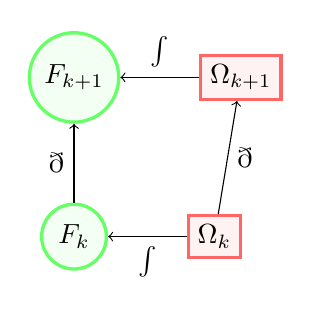
\begin{tikzpicture}
[roundnode/.style={circle, draw=green!60, fill=green!5, very thick, minimum size=7mm},
squarednode/.style={rectangle, draw=red!60, fill=red!5, very thick, minimum size=5mm},
]
\node[roundnode]	(f2) {$F_{k+1}$};
\node[roundnode]	(f1) [below=of f2]{$F_k$};
\node[squarednode]	(w2) [right=of f2] {$\Omega_{k+1}$};
\node[squarednode]	(w1) [right=of f1] {$\Omega_k$};

\draw[<-] (f2) -- (w2) node[midway, above] {$\int$};
\draw[<-] (f2) -- (f1) node[midway, left] {$\eth$};
\draw[<-] (f1) -- (w1) node[midway, below] {$\int$};
\draw[<-] (w2) -- (w1) node[midway, right] {$\eth$};
\end{tikzpicture}


\begin{defn}
	\textbf{Stoke's Theorem}: For (k-1)-form $\omega$ and k-surface $\sigma$, $\int_{\partial \sigma}\omega = \int_{\sigma}\eth\omega$. 
\end{defn}

NOTE: It seems that we don't even needs to worry about orientation as long as we're in coordinate free space. If possible, it would be cool to be able to not talk about orientation at all. It's just a choice of sign on both the direction of integration and the k-form. We can show that changing the sign of the integration necessitates also changing the sign of the k-form, thus making the orientation itself unnecessary (may not be needed). "suppose that you have a k-form, and you have chosen your coordinates, you can switch the order of integration and put a minus on the form, but then components of hte form change, so the form has different components dependign on orientation." "Or, we can say that there is some coordinate for which we go from a to be and others from b to a, components are thus the same, coordinates are different, but make up a class. It's just a different way to keep track of the sign." Components flip sign under a mirror, or flip, or whatever. 

NOTE: If we can stay coordinate free up until this point, maybe we can start talking about coordinates here in the coordinate transformation section
\section{Tensors and coordinate transformations}
Some quantities can undergo one-to-one transformations between coordinate systems. In general, such quantities are tensors. 


\begin{defn}
	A \textbf{tensor} is an object with a one-to-one relationship with objects between coordinate systems. 
\end{defn}

\begin{coro}
	A contravariant tensor of \textbf{rank 1} is a vector, which transforms as  $X'^a = \frac{\partial x'^a}{\partial x^b} X^b$.  
\end{coro}

\begin{coro}
	A covariant tensor of \textbf{rank 1} is a vector, which transforms as $X'_a = \frac{\partial x^b}{\partial x'^a} X_b$. 
\end{coro}

\begin{coro}
	A contravariant tensor of \textbf{rank 2} is a matrix $X^{ab}$ that transforms as $X'^{ab} = \frac{\partial x'^a}{\partial x^c} \frac{\partial x'^b}{\partial x^d} X^{cd}$. 
\end{coro}

\begin{coro}
	A contravariant tensor of \textbf{rank 0} is a quantity $X$ that transforms $X' = X$. Hence, a scalar. 
\end{coro}

- In general, objects associated with covariant tensors will have a lower index, and those associated with contravariant tensors will have an upper index. 












\chapter{Geometry and (States, Tensors, Forms)???}


\section{Symplectic geometry and state spaces}
We want to be able to represent our state configurations. Symplectic geometry arises when trying to describe their areas

\subsection{Symplectic form and areas}



\subsection{Metric tensor}
A more generalized inner product: feed in two vectors, and the outcome is a scalar representing the lengths of the vectors and the angle between them. 

\begin{defn}
	A \textbf{metric tensor g} is a function that takes two vectors and returns a real scalar. 
\end{defn}


\section{Riemannian geometry}
In order to give a mathematically rigorous definition of lengths of vectors and the angle between them, we use an inner product. Vector spaces with an inner product are Riemannian.

\begin{defn}
	Given two vectors $X^a,Y^a \in V$ and a metric tensor $g_{ab}$, the \textbf{inner product} $<X^a,Y^a> : V \times V \to \mathbb{R}$ is defined as $<X^a,Y^a> = g_{ab}X^aY^b$. 
\end{defn}

\begin{coro}
	The magnitude of $<u,v>$ is $|u||v|cos(\theta)$, where $\theta$ is the angle between u and v. 
\end{coro}

\begin{defn}
	If a vector space V contains an inner product, then V is \textbf{Riemannian}.
	\end{defn}



\subsection{Orthogonal basis}

\begin{defn}
	For contravariant vectors $X^a$ and $Y^a$, the two vectors are \textbf{orthogonal} if $<X^a,Y^b> = 0$. 
\end{defn}







\end{document}